% Copyright (c) 2013 Joost van Zwieten

% Permission is hereby granted, free of charge, to any person obtaining a copy
% of this software and associated documentation files (the "Software"), to deal
% in the Software without restriction, including without limitation the rights
% to use, copy, modify, merge, publish, distribute, sublicense, and/or sell
% copies of the Software, and to permit persons to whom the Software is
% furnished to do so, subject to the following conditions:

% The above copyright notice and this permission notice shall be included in
% all copies or substantial portions of the Software.

% THE SOFTWARE IS PROVIDED "AS IS", WITHOUT WARRANTY OF ANY KIND, EXPRESS OR
% IMPLIED, INCLUDING BUT NOT LIMITED TO THE WARRANTIES OF MERCHANTABILITY,
% FITNESS FOR A PARTICULAR PURPOSE AND NONINFRINGEMENT. IN NO EVENT SHALL THE
% AUTHORS OR COPYRIGHT HOLDERS BE LIABLE FOR ANY CLAIM, DAMAGES OR OTHER
% LIABILITY, WHETHER IN AN ACTION OF CONTRACT, TORT OR OTHERWISE, ARISING FROM,
% OUT OF OR IN CONNECTION WITH THE SOFTWARE OR THE USE OR OTHER DEALINGS IN
% THE SOFTWARE.
%
\documentclass{tudelftposter}

% optional, makes QR code clickable
\usepackage[implicit=false,bookmarks=false]{hyperref}
\usepackage[utf8]{inputenc} % allow utf-8 input
\usepackage[T1]{fontenc}    % use 8-bit T1 fonts
\usepackage{url}            % simple URL typesetting
\usepackage{booktabs}       % professional-quality tables
\usepackage{amsfonts}       % blackboard math symbols
\usepackage{nicefrac}       % compact symbols for 1/2, etc.
\usepackage{microtype}      % microtypography
\usepackage{lipsum}
\usepackage{listings}
\usepackage{amsmath}
\usepackage{diagbox}
\usepackage{tabularx}
\usepackage{longtable}
\lstset{language = C}
\usepackage{graphicx,changepage}
\usepackage{float}
\usepackage{graphicx}
\usepackage{kotex}
\usepackage{xcolor}
\usepackage{color}
\usepackage{caption}
\usepackage{minted}
\usepackage{svg}
\usepackage{cclicenses}
\usepackage{tikz}
\usetikzlibrary{positioning}

\definecolor{mybluei}{RGB}{124,156,205}
\definecolor{myblueii}{RGB}{73,121,193}
\definecolor{mygreen}{RGB}{202,217,126}
\pgfdeclarelayer{background}
\pgfsetlayers{background,main}


\usepackage{setspace}

\hypersetup{%
  colorlinks=true,% hyperlinks will be black
  linkbordercolor=red,% hyperlink borders will be red
  pdfborderstyle={/S/U/W 2}% border style will be underline of width 1pt
}


\onehalfspacing
\graphicspath{./img/}
\title{마인크래프트 강화학습 환경 구축을 통한 멀티모달 연구\\
\large 와 특정 태스크에서의 우수성 비교}

\addauthornote{mail}[@]{\ttfamily yhs0602@snu.ac.kr}
% \addauthornote{diam}{Delft Institute of Applied Mathematics, TU Delft}
% \addauthornote{tp}{Department of Theoretical Physics, TU Delft}

% \addauthor[mail,diam]{J.F. Nash}
% \addauthor[diam,tp]{C.F. Gau{\ss}}
\addauthor{2019-13674 양현서 / 지도교수 장병탁}
% \addauthor[tp]{R.P. Feynman}

% \addfootimage(c:right column.center)[Delft Institute of Applied Mathematics]{tudelft}
% \ifqrcodessupported
%   % NOTE: compile this document with lualatex instead of pdflatex
%   \addfootqrcode(l:left column.left)[tudelft-poster repository]{http://github.com/joostvanzwieten/tudelft-poster}
% \else
%   \addfootobject*(l:left column.left)[research web page]{%
%     \begin{tikzpicture}
%       \node[red,draw,inner sep=1ex] {%
%         \begin{minipage}{15cm}
%           \footnotesize%
%           Please compile this document with lualatex to see a QR code here:\\
%           \null\texttt{\quad lualatex \jobname}
%         \end{minipage}};
%     \end{tikzpicture}}
% \fi

\begin{document}

% \SetSerifFonts{gt}{gt}
% \SetSansFonts{mj}{mj}
\section{서론}
\subsection{연구 주제}
강화학습을 위한 마인크래프트 환경에서 어둠 상태 효과를 활용한 시야 제한 태스크와 멀티모달 정보 활용의 중요성

\subsection{연구 동기 및 목적}
강화학습 연구의 다양한 도메인에 대한 새로운 환경의 필요성을 제기하고, 마인크래프트를 활용하여 이를 구축할 수 있는 가능성을 제시한다. 또한 이 새로운 환경에서 이용 가능한 어둠 상태 효과를 활용하여 시야가 제한된 상황에서의 태스크를 제시한다. 이 때 기존 비전 기반 모델이나 음원 방향 정보만 이용한 모델과 달리 비전 정보와 소리 정보를 모두 활용한 멀티모달 모델을 제시하여 성능을 비교한다. 이를 통해 강화학습 태스크에서 멀티모달 정보의 활용의 중요성을 강조한다.

\section{이론적 배경}
\subsection{강화학습}
강화학습은 에이전트가 환경과 상호작용하며, 보상을 최대화하는 행동을 학습하는 방법이다. 강화학습의 학습 과정은 다음 그림에서 볼 수 있다.

\begin{figure}
  \centering
  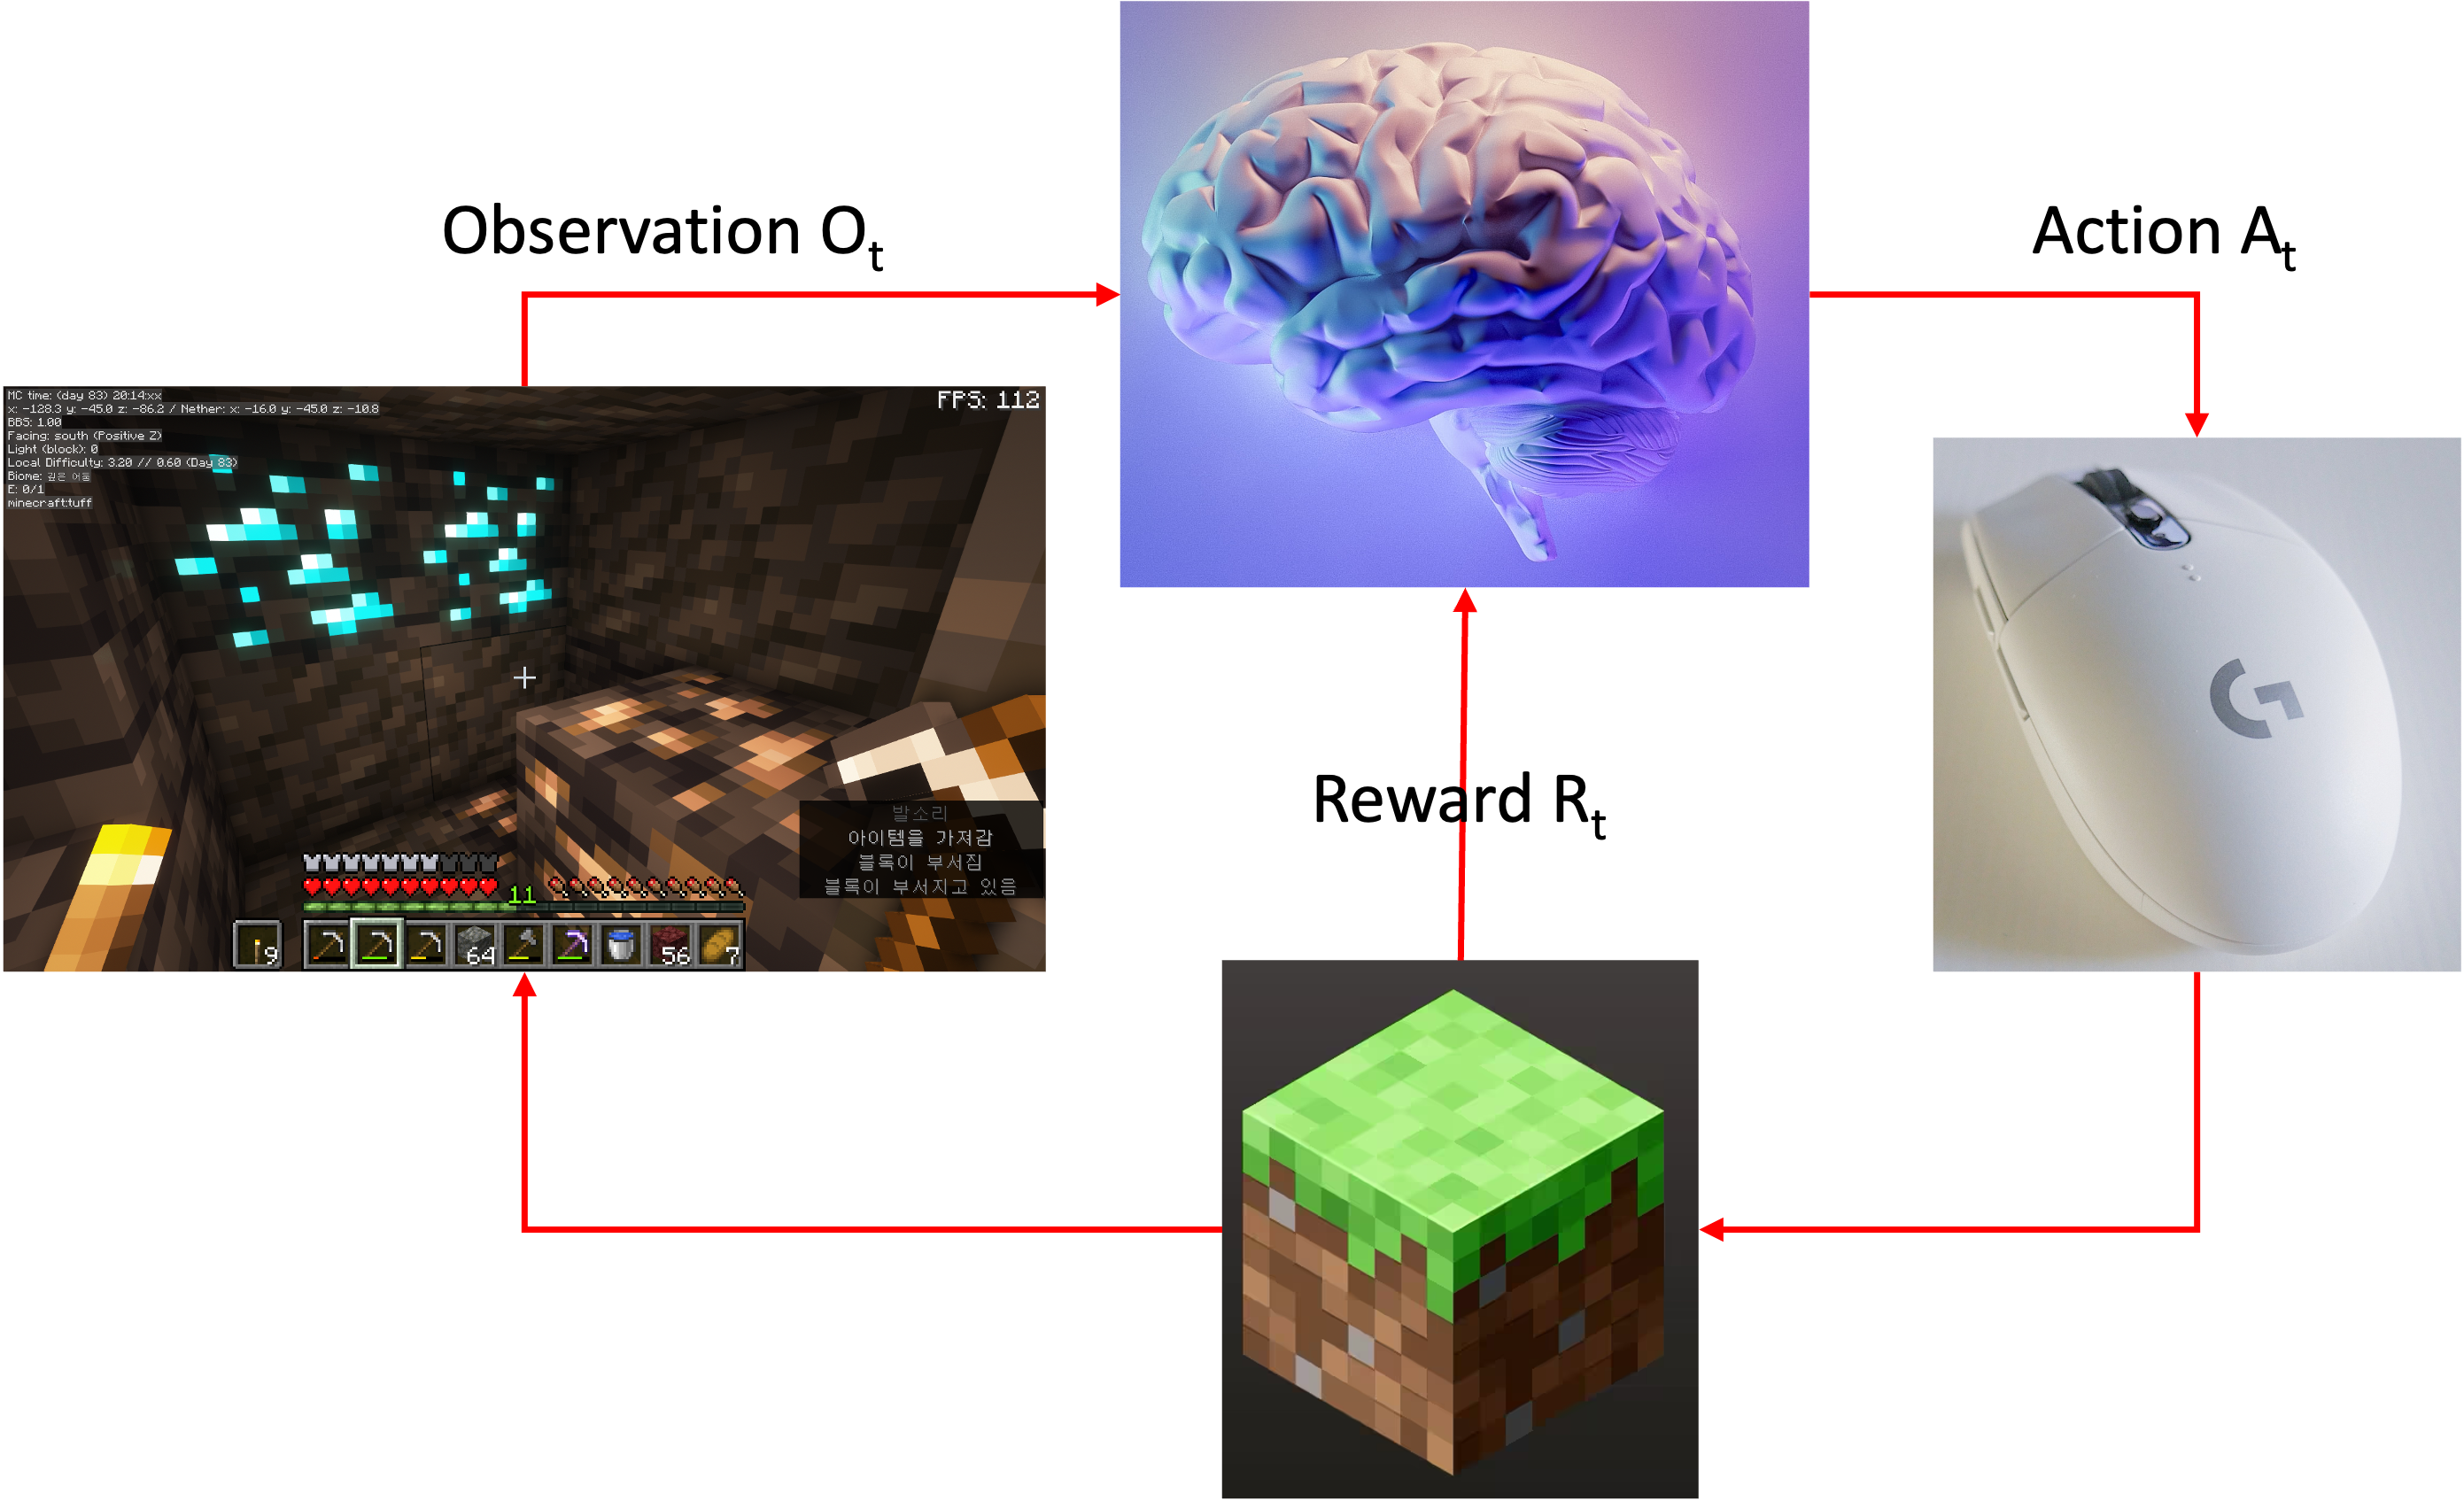
\includegraphics[width=.35\textwidth]{reinforcement.png}
  \caption{강화학습의 학습 과정. 에이전트는 Observation $O_t$를 받아 Policy $\pi_\theta$에 따라 Action $A_t$를 선택하고, Environment는 Reward $R_t$와 다음 Observation $O_{t+1}$을 반환한다.}
  \label{fig:reinforcement}
\end{figure}
강화학습 에이전트는 어떤 시점 t에서의 observation $O_t$를 받아 policy $\pi_\theta$에 따라 action $A_t$를 선택하고, environment는 reward $R_t$와 다음 observation $O_{t+1}$을 반환한다. 이러한 과정을 반복하면서 에이전트는 보상을 최대화하는 policy를 학습한다. 본 연구에서는 강화학습 알고리즘 중 하나인 DQN을 사용한다. DQN은 심층 신경망을 활용하여 어떤 상태 $s$, 즉 $O_t$에서 어떤 행동 $a$를 취했을 때의 가치 $Q(s,a)$를 추정한다. 이러한 추정을 통해 에이전트는 가치가 높은 행동을 선택하도록 학습한다. 이를 통해 에이전트는 기대되는 보상의 총합이 가장 큰 행동을 선택할 수 있게 된다. DQN은 다음과 같은 손실 함수를 최소화하는 방향으로 학습된다.
\begin{equation}
  L(\theta) = \mathbb{E}_{s,a,r,s' \sim D}[(r + \gamma \max_{a'}Q(s',a';\theta^-) - Q(s,a;\theta))^2]
\end{equation}
여기서 $D$는 경험의 집합이며, $\theta$는 현재 네트워크의 파라미터, $\theta^-$는 타겟 네트워크의 파라미터, $\gamma$는 감가율이다. 감가율이란 에이전트가 미래의 보상을 현재의 보상에 비해 얼마나 중요하게 생각하는지에 대한 요소이며, 일반적으로 0과 1 사이의 값이다. 이 손실 함수는 현재 네트워크의 추정 가치와 타겟 네트워크의 추정 가치의 차이를 최소화하는 방향으로 학습된다. 이것을 TD 오차라고 하며, DQN은 학습이 진행됨에 따라 일정 주기로 타겟 네트워크의 파라미터 $\theta^-$를 현재 네트워크의 파라미터 $\theta$로 업데이트한다.

\section{연구 방법}
\subsection{Environment}
Minecraft를 인간이 아닌 프로그램으로 조작하기 위해서 ``모드''라는 기능을 활용하였다. 모드를 이용하면 게임을 수정할 수 있다. 이를 통해 파이썬으로 작성된 에이전트가 게임을 조작할 수 있게 게임을 수정하였다.

\begin{figure}
  \centering
  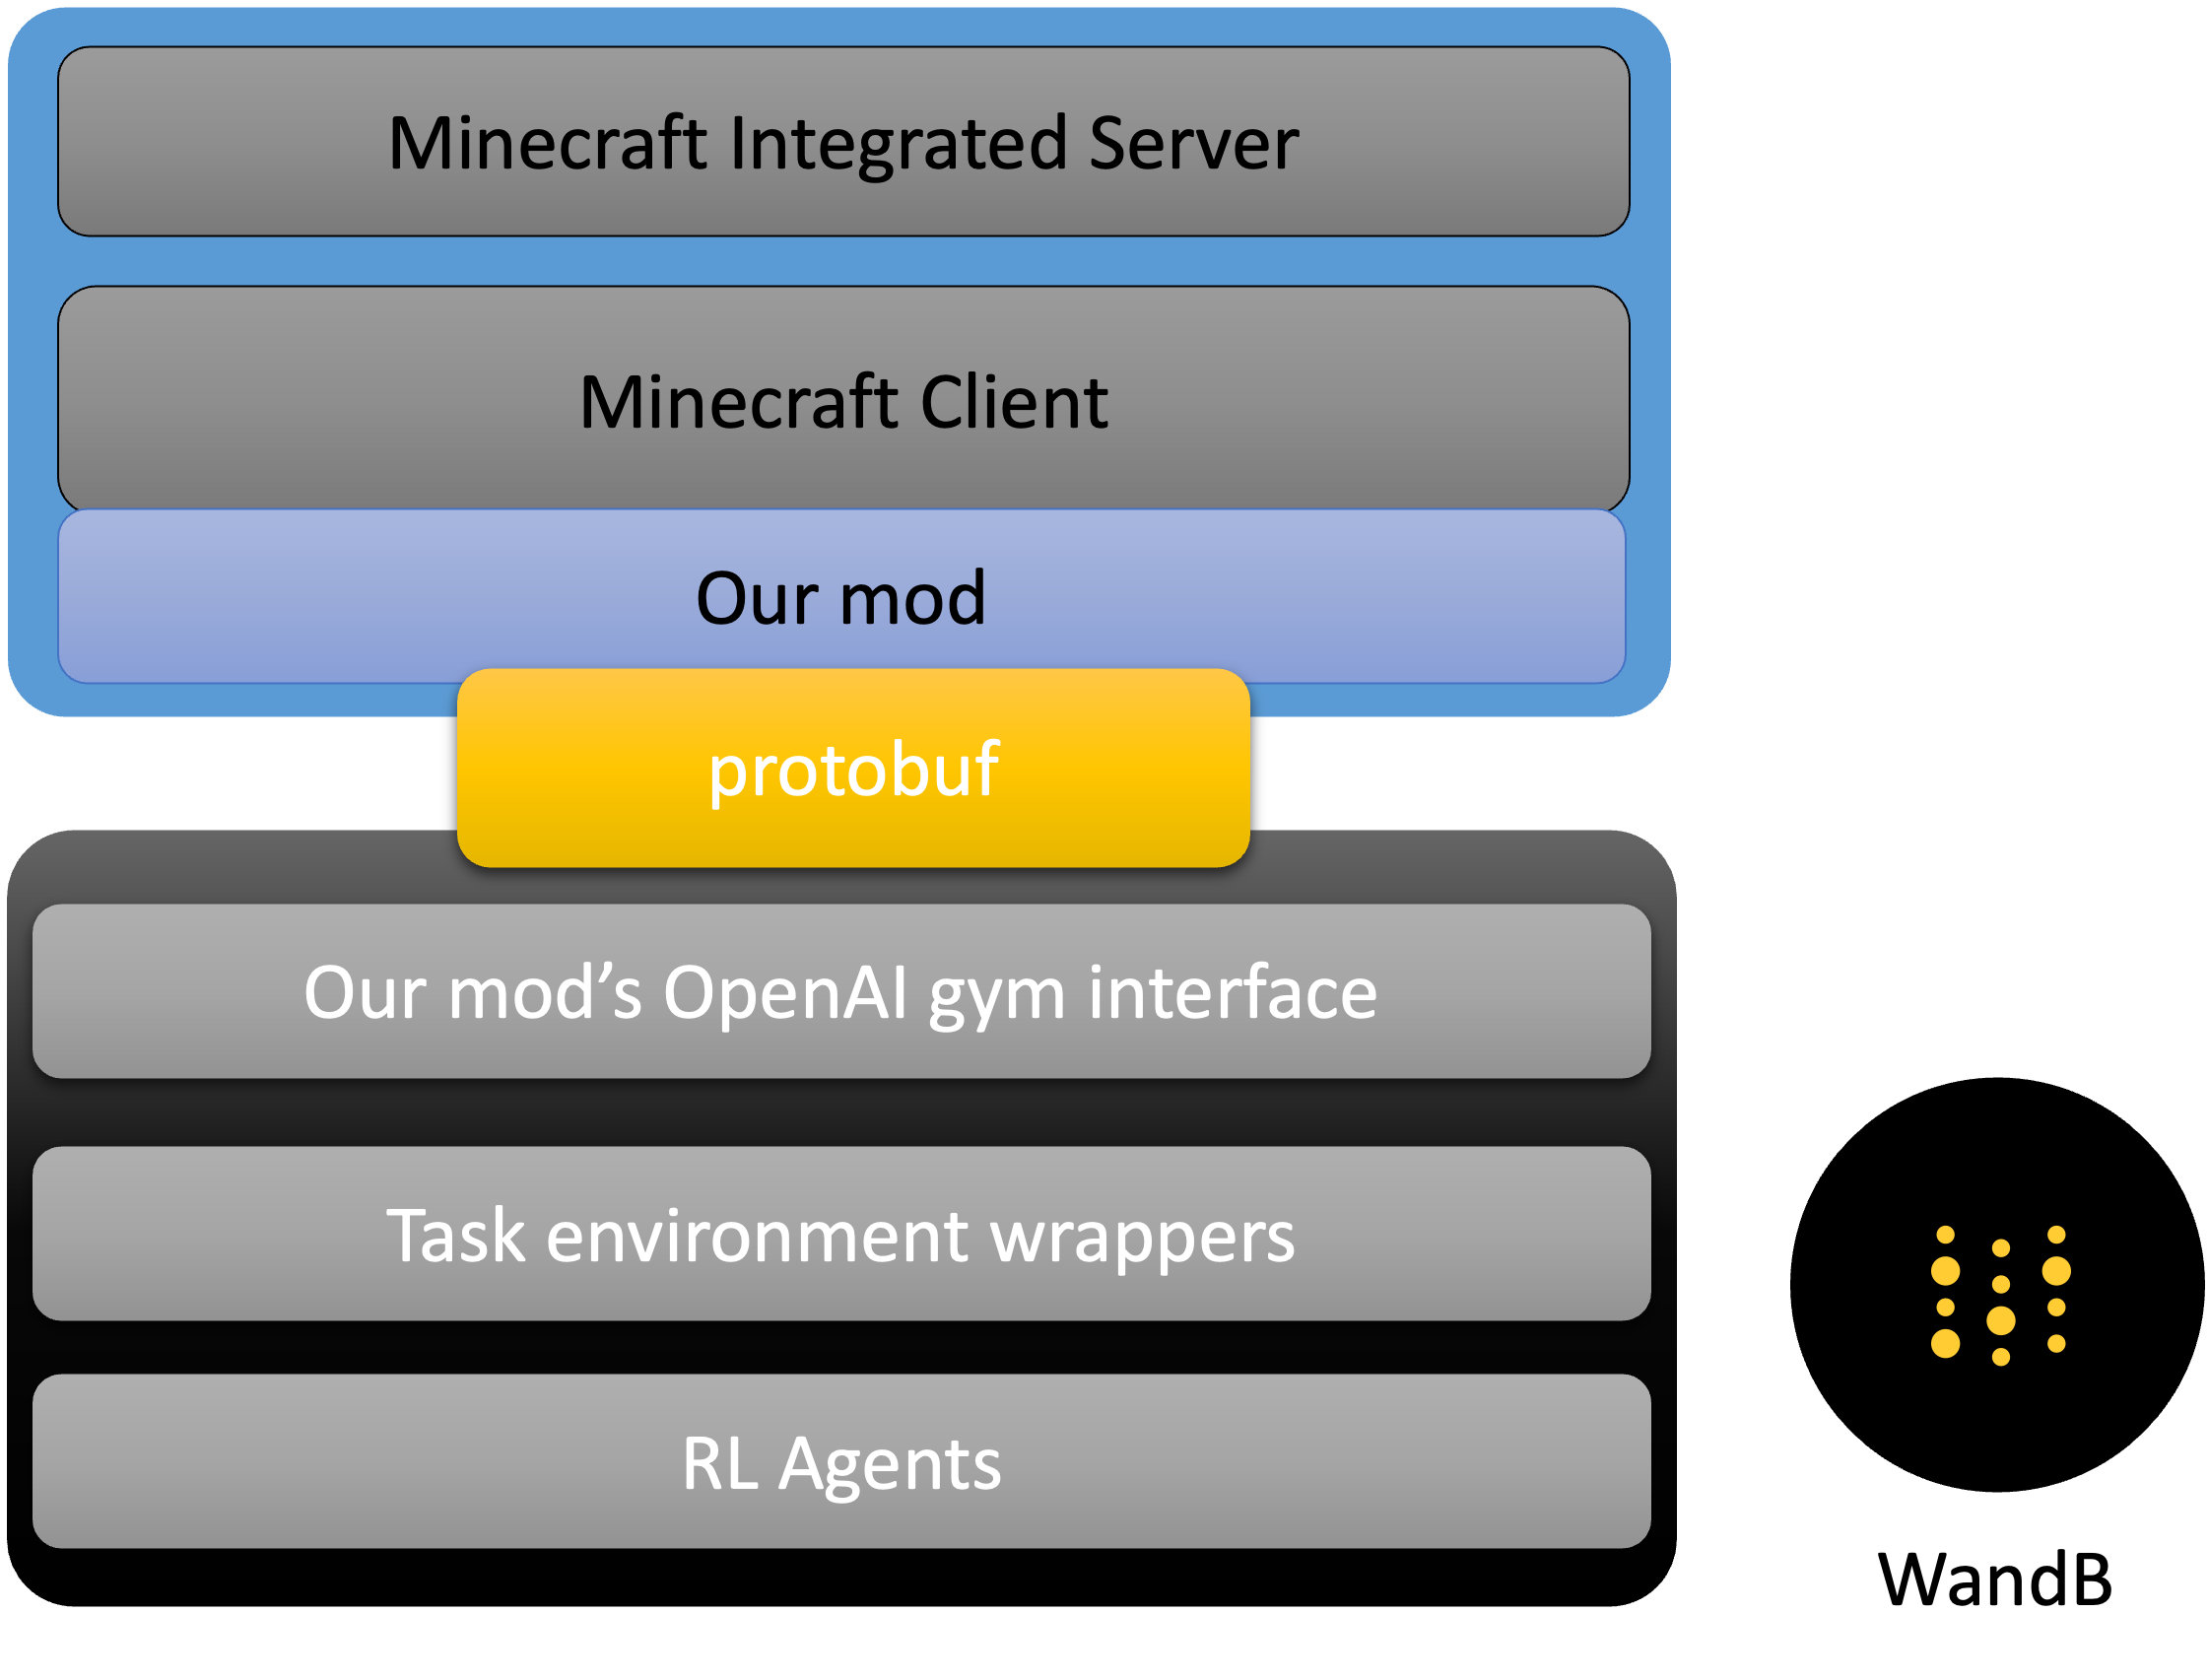
\includegraphics[width=.3\textwidth]{arch1.png}
  \caption{환경을 나타내는 그림. 강화학습 에이전트가 env.reset이나 step을 호출하면, 우리의 wrapper는 마인크래프트를 실행한 후, protobuf over TCP를 통해 우리의 마인크래프트 모드와 통신한다. 마인크래프트 모드는 플레이어를 조작하고, 관측 공간을 캡처하여 wrapper에게 전달한다. wrapper는 관측 공간을 처리하여 강화학습 에이전트에게 전달한다.}
  \label{fig:test}
\end{figure}


\subsection{태스크 설계}
실험은 1개의 태스크와 3개의 모델을 이용하여 진행하였다. 먼저 태스크는 다음과 같다. 
\begin{itemize}
  \item 완전한 평지 지형에서 어둠 상태 효과가 걸린 상태에서 한 마리의 허스크를 피해 도망가기
\end{itemize}
허스크란 마인크래프트에서 좀비의 변종으로, 플레이어를 추적해 공격하며, 태양빛에 면역인 특징이 있다. 게임 속의 낮에 실험하기 용이하여 좀비 대신 허스크를 선택하였다. 어둠 상태 효과란 플레이어의 시야를 극도로 어둡게 만드는 상태 효과로서, 가까운 거리 이외의 시야를 어둠으로 차단한다.

\subsection{모델 설계}
\begin{figure}
  \centering
  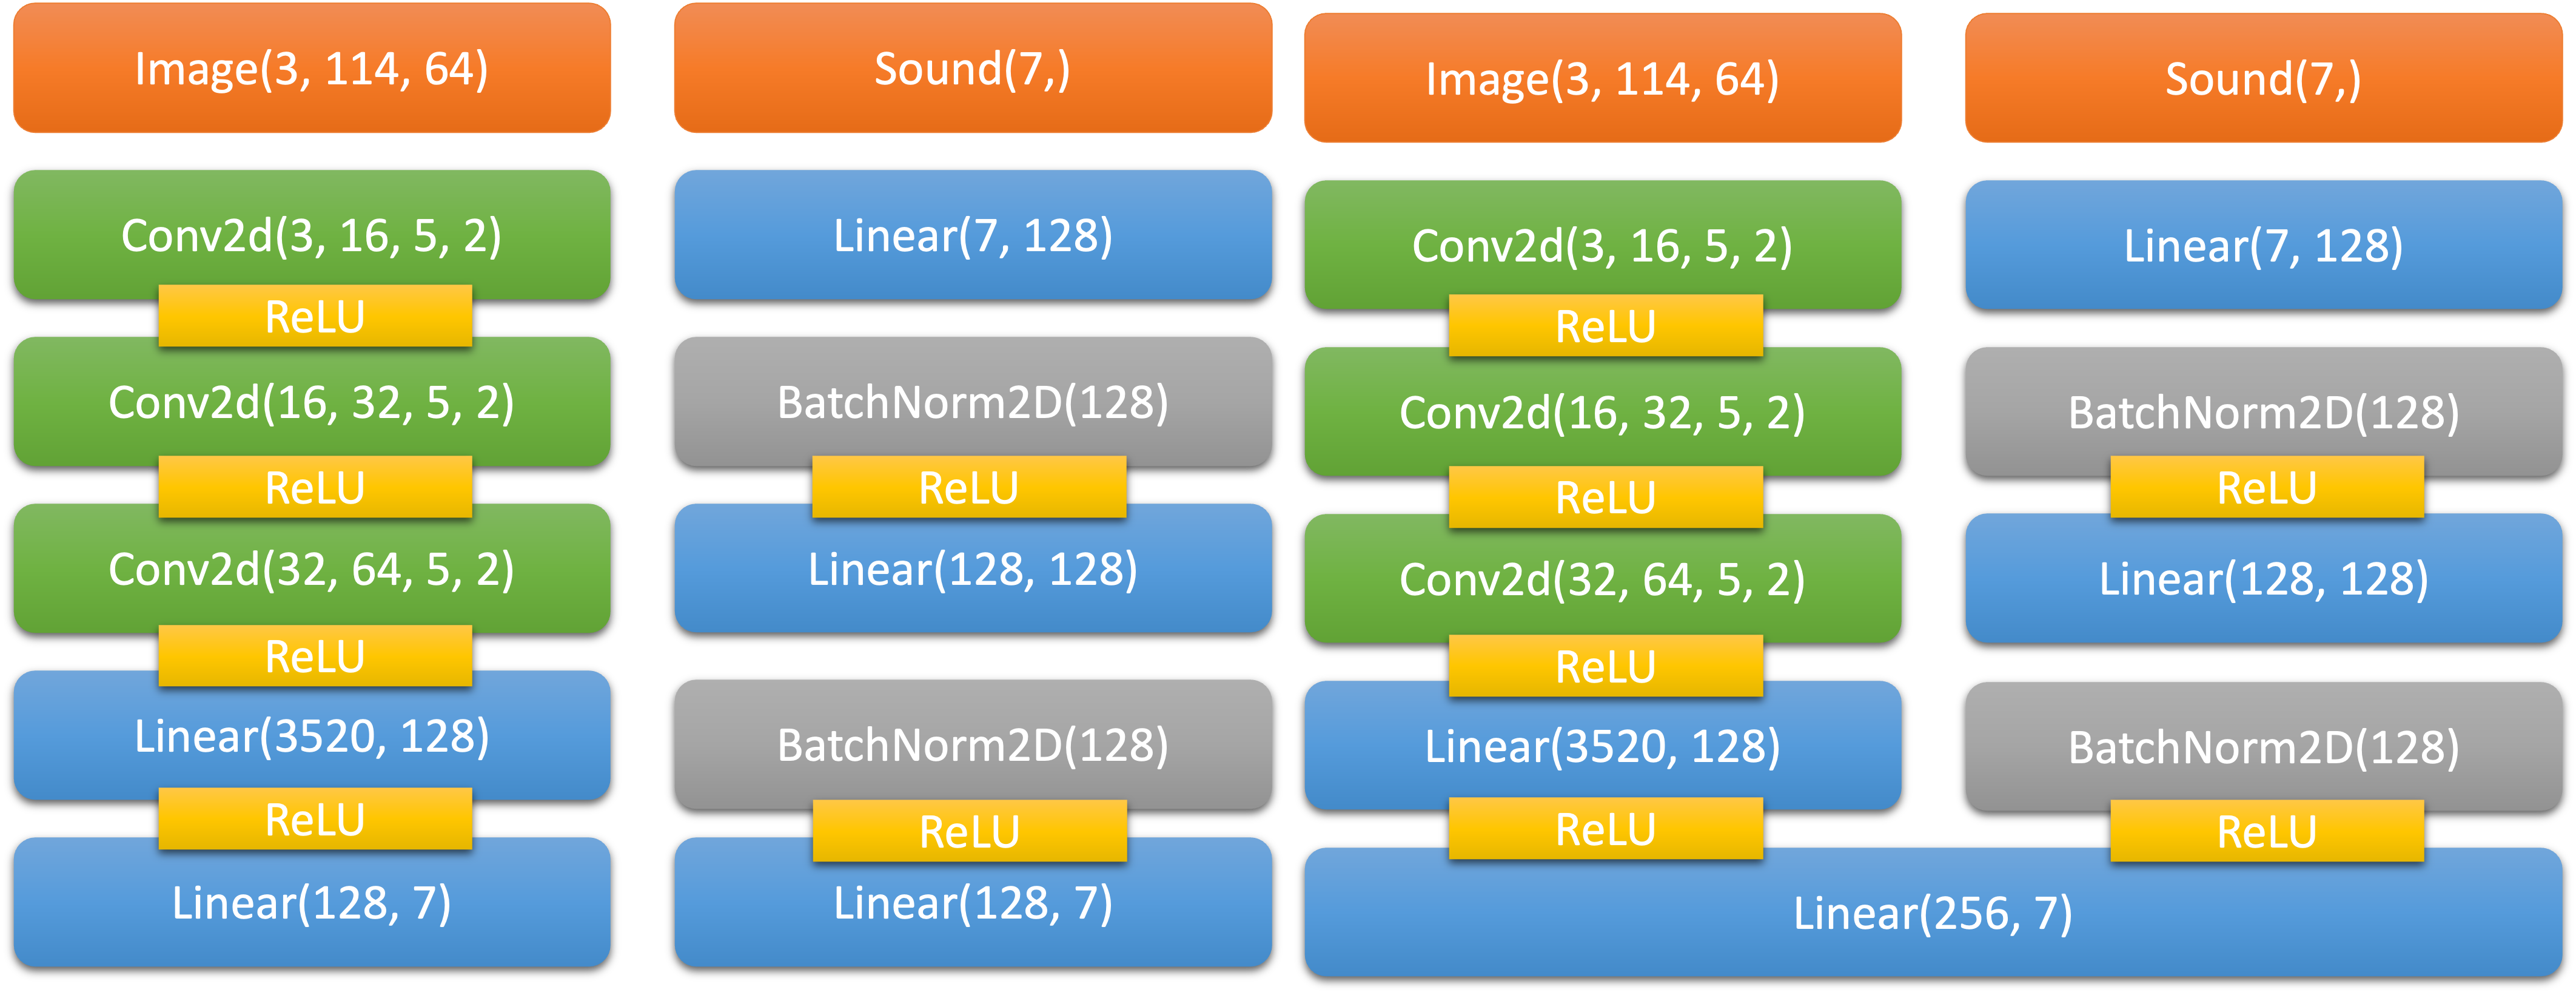
\includegraphics[width=.45\textwidth]{models.png}
  \caption{실험에 사용된 네트워크의 구조도. 왼쪽부터 시각 정보를 이용하는 에이전트, 소리와 방향 정보를 이용하는 에이전트, 멀티모달 에이전트이다. Conv2d의 숫자들은 왼쪽부터 입력 채널 수, 출력 채널 수, 커널 크기, stride를 의미한다. Linear의 숫자들은 왼쪽부터 입력 차원 수, 출력 차원 수를 의미한다.}
  \label{fig:models}
\end{figure}
비전 입력의 경우, 게임 화면을 매 시뮬레이션 단위(틱)마다 캡처하여 에이전트에 전달한다. 음원 위치 입력의 경우, 우리 환경에서 에이전트에 대한 음원의 상대 좌표와 종류를 알아낼 수 있다. 해당 상대 좌표 벡터를 정규화하고, 현재 에이전트가 바라보고 있는 방향은 방향의 주기성을 고려하여 cos와 sin을 취해 입력했다. 완전한 평지 지형에서 테스트하므로, 에이전트와 허스크의 상대 y좌표는 항상 0이므로 입력에서 제외하였다. 플레이어가 허스크에게 공격받아 나는 소리는 항상 상대좌표가 0이므로, 0과 1로만 표시하였다. 이렇게 7차원 벡터를 입력으로 제공하였다.

\subsection{보상 설계}
에이전트에게 매 시간 단위(틱)마다 아래의 보상을 부여하였다.
\begin{itemize}
  \item 살아 있을 경우 0.5
  \item 죽었을 경우 -1
\end{itemize}
에피소드마다 400틱이 지나거나, 허스크에게 죽을 경우 시뮬레이션을 중단하였다. 따라서 에이전트가 한 에피소드에서 받을 수 있는 보상의 최대값은 200이다.

\section{연구 결과}

\begin{figure}
  \centering
  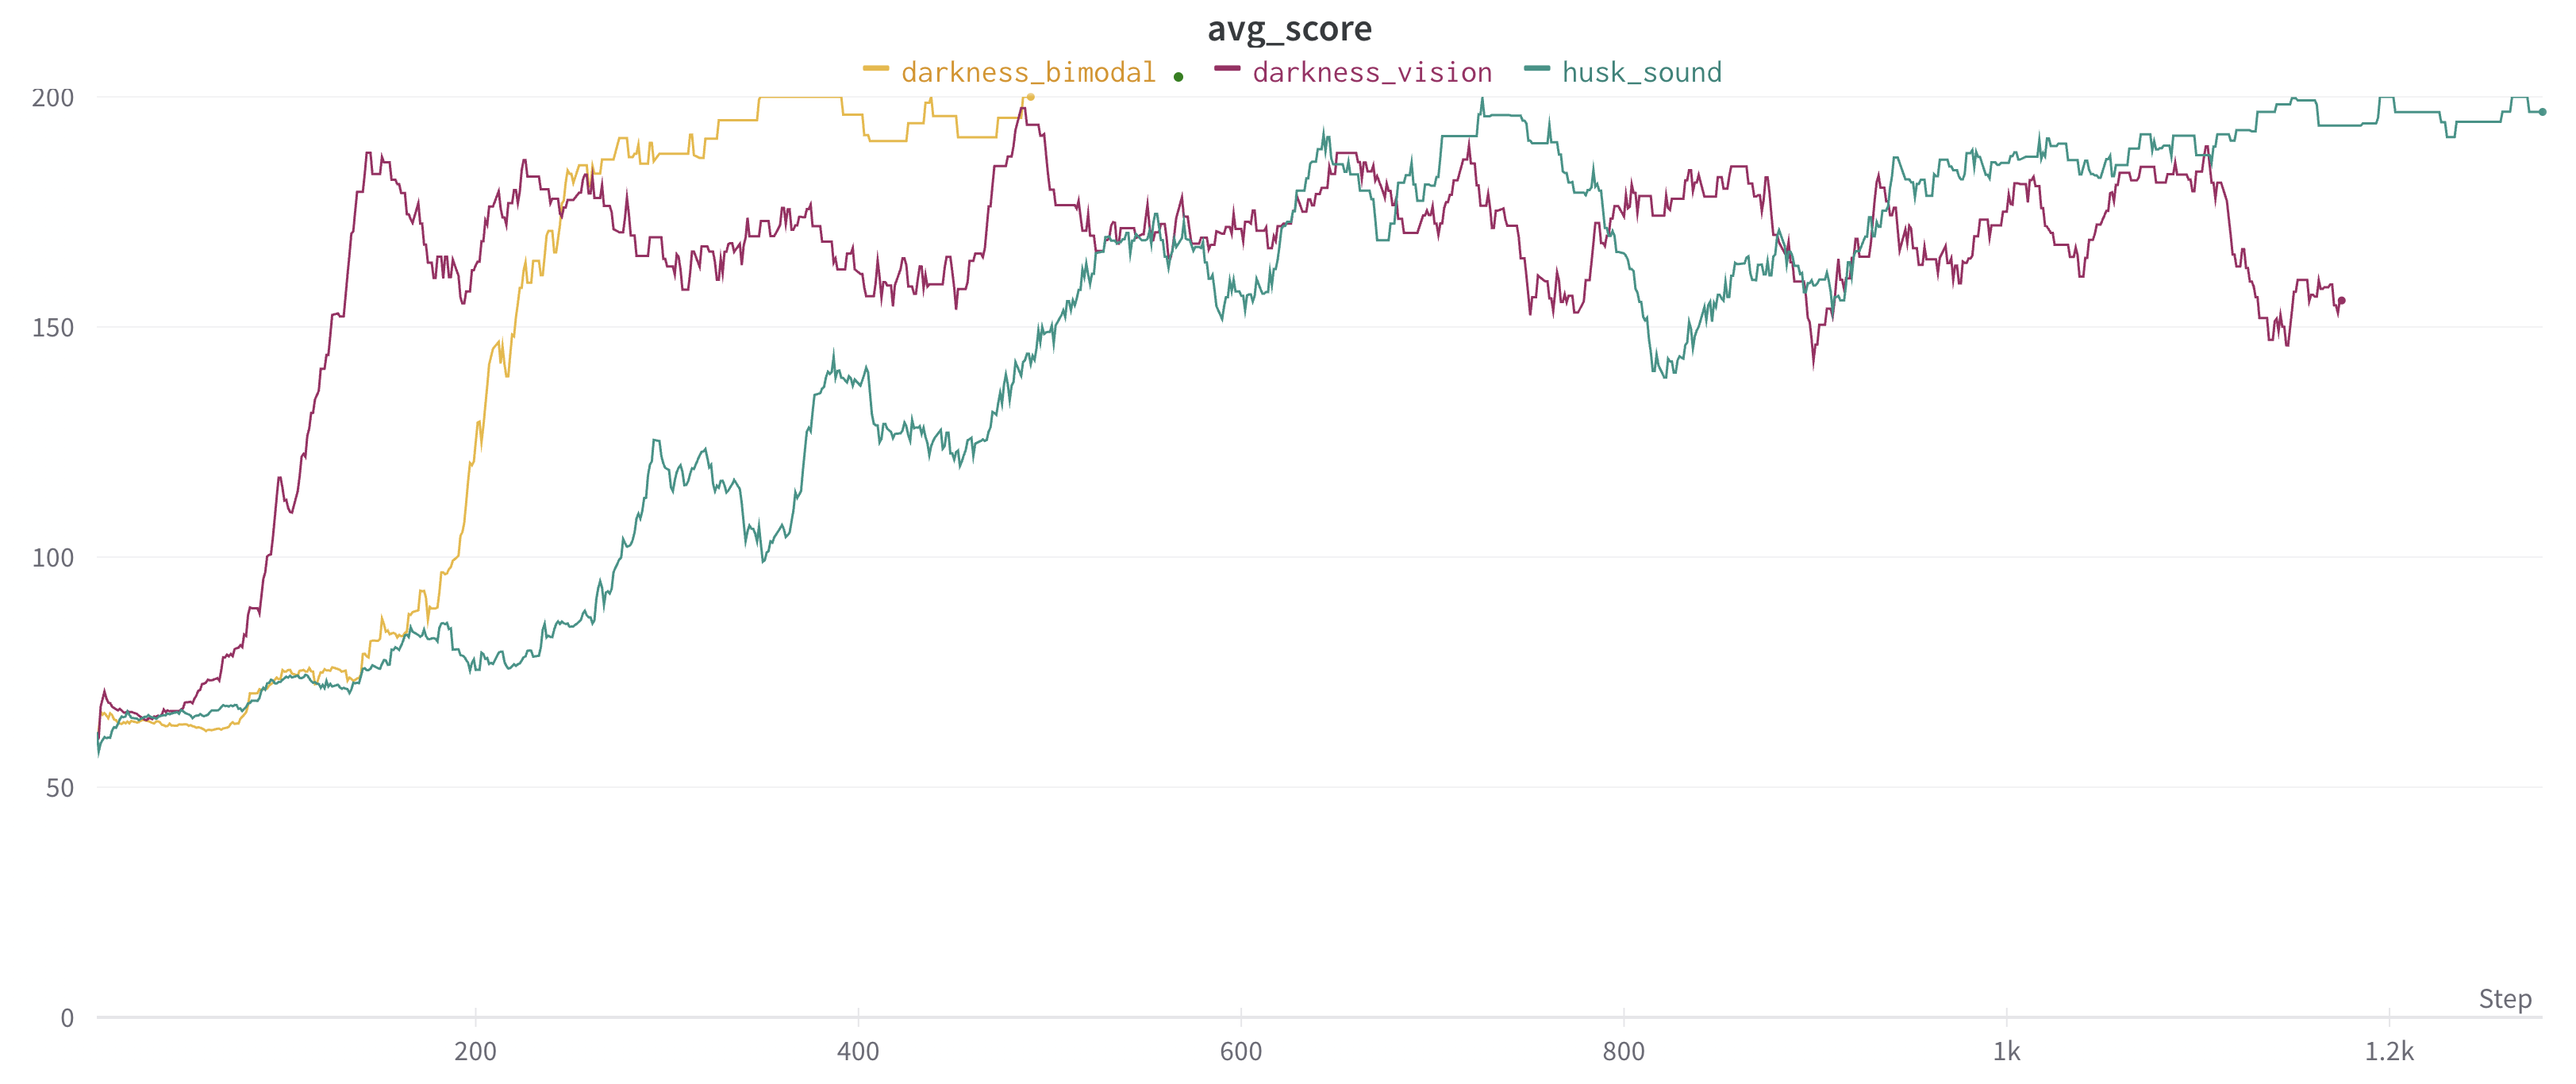
\includegraphics[width=.5\textwidth]{result.png}
  \caption{어둠 상태 효과를 받은 상태에서 플레이어를 추적하여 공격하는 몬스터인 허스크를 회피하는 태스크를 수행한 에이전트들의 학습 곡선. 자주색은 $3\times114\times64$의 게임 화면 입력을 받아 7가지 액션 (전진, 후진, 왼쪽으로 이동, 오른쪽으로 이동, 왼쪽으로 15도 회전, 오른쪽으로 15도 회전, 정지)중 하나를 선택한다. 마찬가지로 초록 곡선은 7차원 소리 벡터를 받아 7가지 액션 중 하나를 선택하는 에이전트의 곡선이고, 노란 곡선은 시각 및 소리 방향 정보를 모두 받아 7가지 액션 중 하나를 선택하는 멀티모달 에이전트의 곡선이다.}
  \label{fig:block}
\end{figure}
실험 결과, 소리만 이용하여 허스크를 피하는 경우, 소리가 가끔씩만 들려오는 특징으로 인해서 학습이 느려졌다. 비전만 이용하여 허스크를 피하는 경우, 플레이어가 허스크를 바라보지 않는 경우 항상 같은 입력을 받는 특징으로 인하여 일정 이상의 성능을 달성하지 못하였다. 시각과 음원 방향 정보를 모두 이용하는 에이전트의 경우, 위 두 정보의 장점을 모두 이용하여 빠른 학습과 높은 학습 성능을 보였다. 이는 앞서 설명한 모델 구조와 같이 상대적으로 단순한 멀티모달 모델이라도 좋은 성능을 보여줄 수 있음을 보여준다.

\subsection{연구 결과 소스 코드 저장소}
\href{https://github.com/KYHSGeekCode/MinecraftRL}{https://github.com/KYHSGeekCode/MinecraftRL}에서 본 포스터의 소스 코드를 탐색할 수 있다.


\section{시사점}
이 연구에서는 강화 학습 환경으로 인기를 얻고 있는 마인크래프트에서의 새로운 학습 환경을 개발했다. 마인크래프트를 강화 학습 환경으로 활용하는 기존 연구들과는 달리 이번 연구에서는 최신 버전인 1.19 이상을 사용하는 환경을 만들었으며, 이를 이용해 어둠 상태 효과가 걸린 상태의 태스크를 해결하는 에이전트를 훈련시켰다. 그 결과, 시각과 음원 방향의 각각의 정보만을 사용하는 에이전트보다, 둘 다의 정보를 이용하는 멀티모달 모델이 좋은 성능을 내는 것을 실험을 통해 검증하였다. 이를 통해 실생활에서는 로봇이 화재 상황이나 야간과 같이 시야가 제한된 상황에서 비전 정보와 더불어 소리 정보도 같이 이용하는 것이 로봇의 효과적인 임무 수행에 도움을 줄 수 있다는 점을 보여주었다.

% \bibliographystyle{unsrt}
% \begin{thebibliography}{1}
%     \bibitem{WDD2009}
%     이봉석, 『윈도우 디바이스 드라이버』, {\em 한빛미디어}, 2009.
% \end{thebibliography}


\end{document}
% vim: tw=80:ts=2:sts=2:sw=2:et:fdm=marker:fmr=[[[,]]]

